% ============================================================
% Appendix for Chapter: ch_nreps2023
% Yang, Sun, Buzsáki. NeurReps / NeurIPS Workshop 2023.
% ============================================================

\subsection*{Appendix A: Nonlinear Dimensionality Reduction for Decoding Replay Events}
\label{app:nreps_A}

\begin{figure}[htbp]
    \centering
    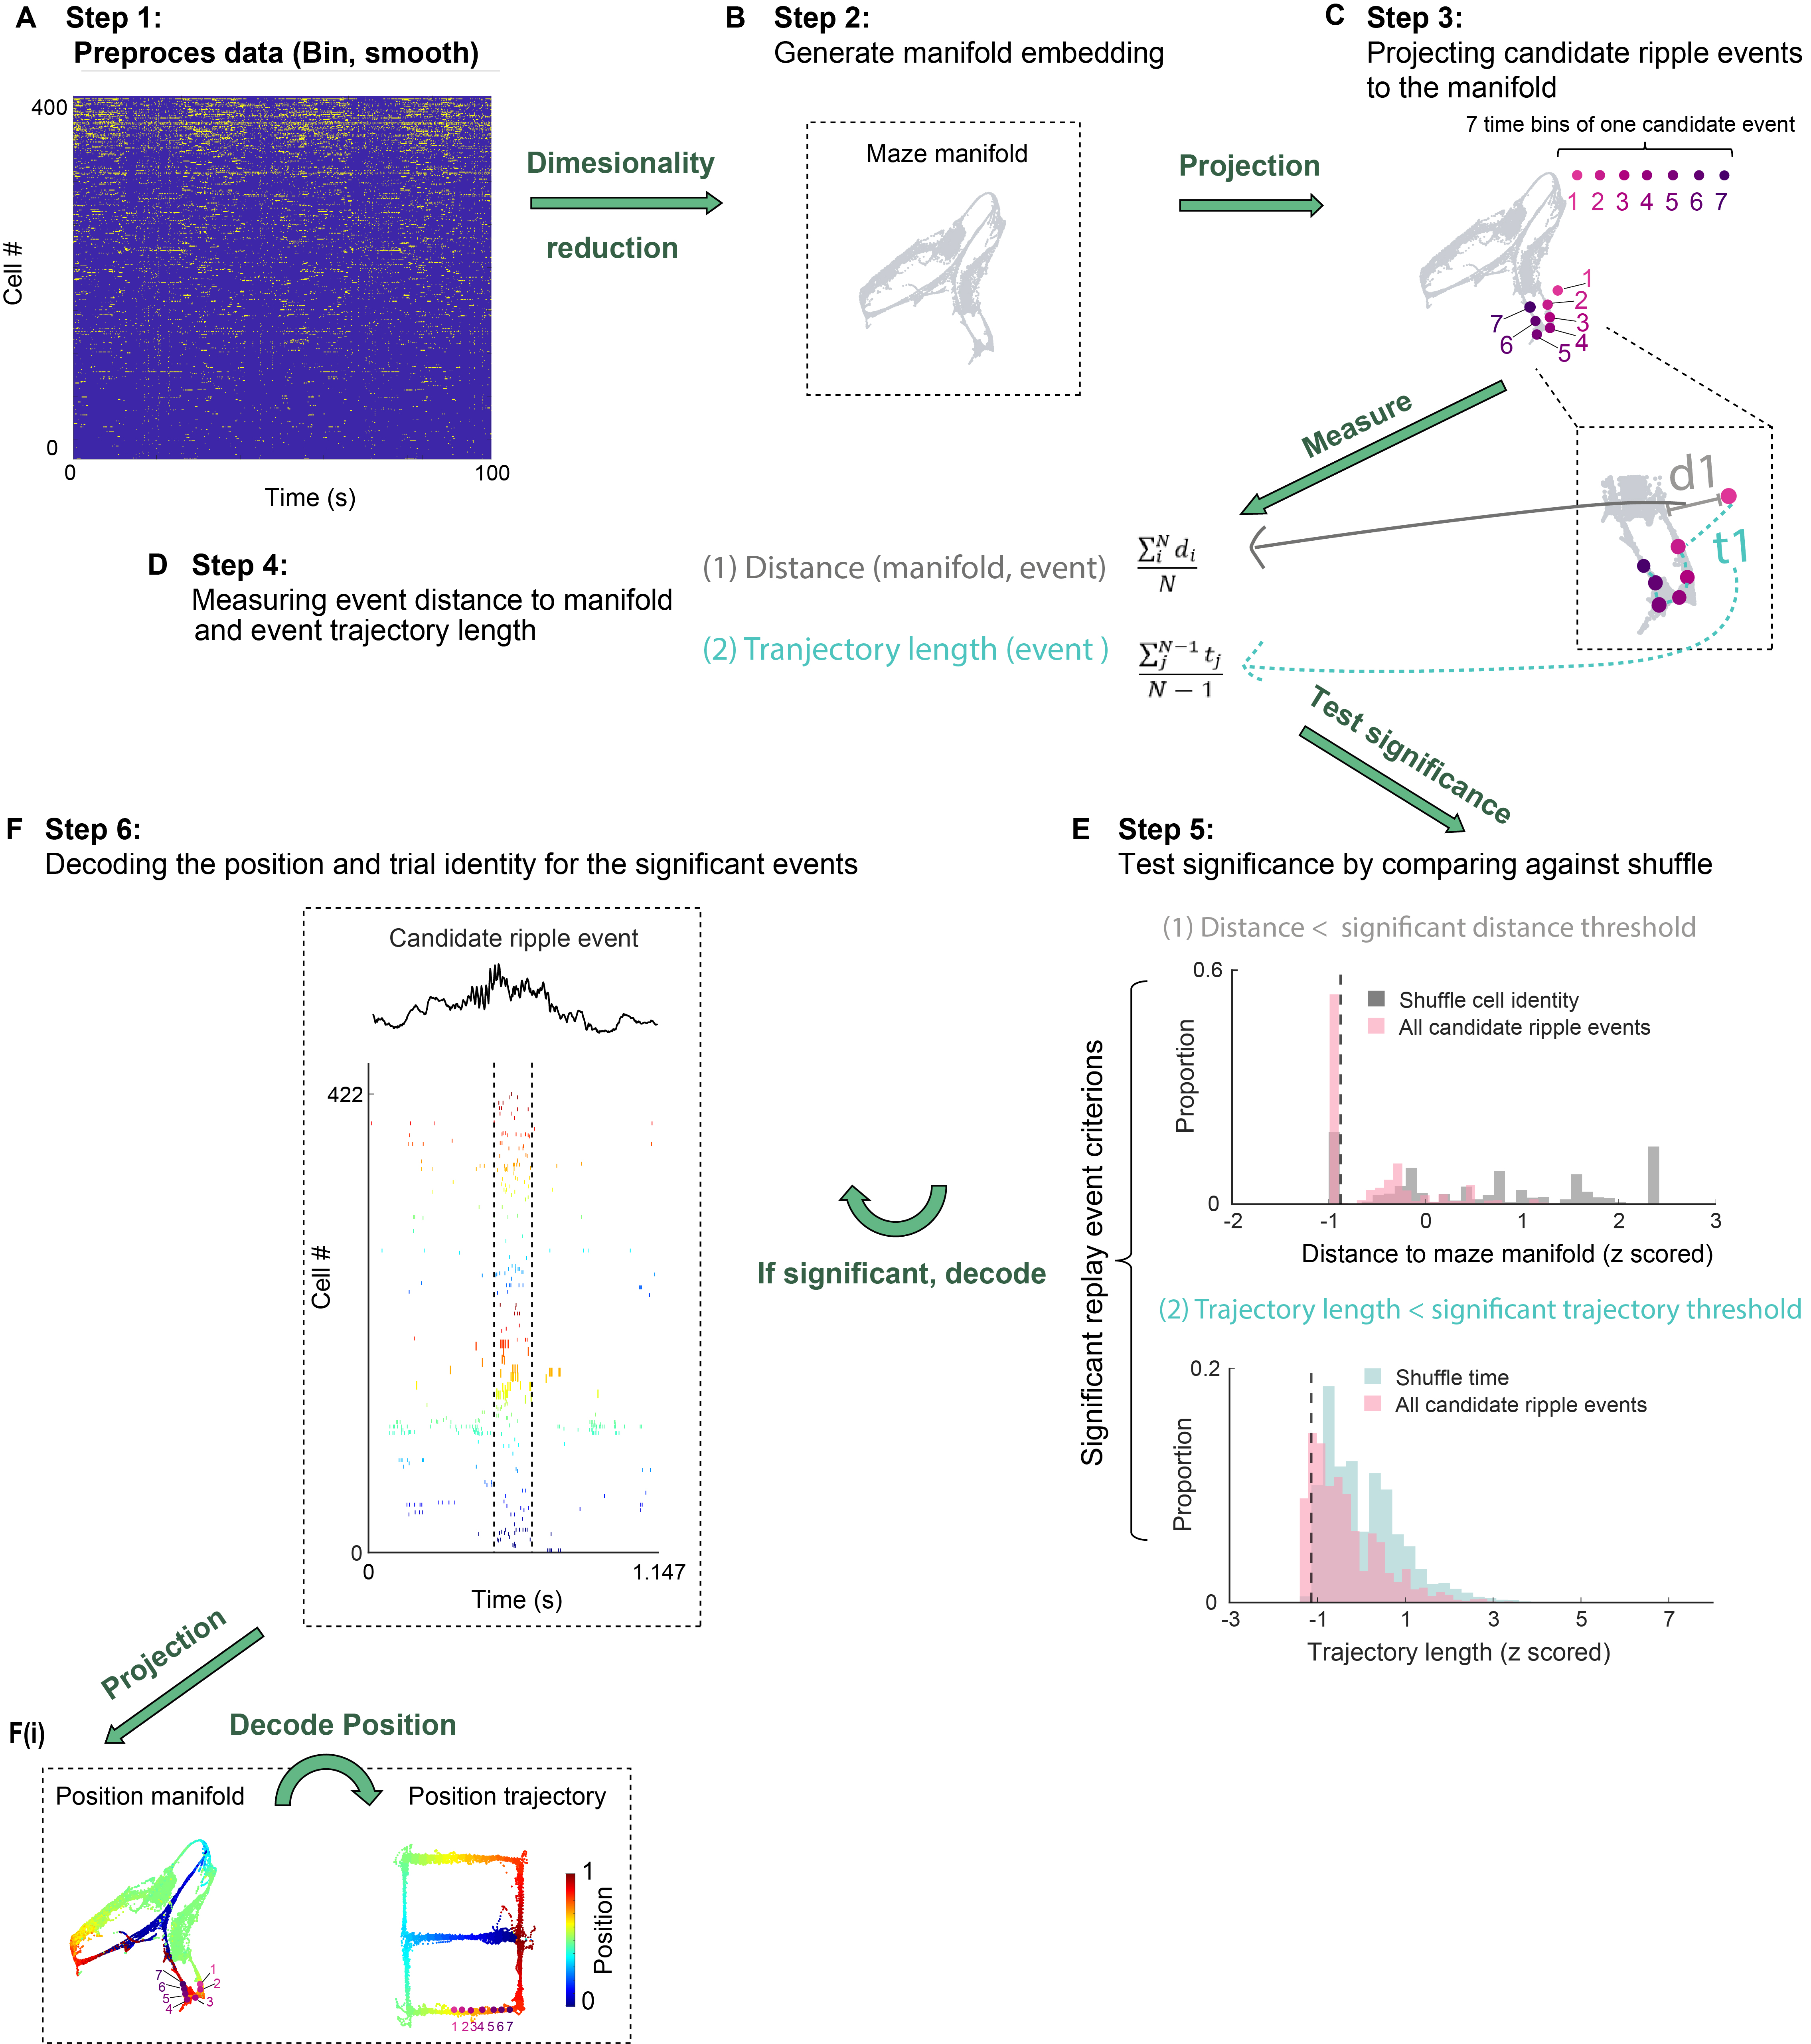
\includegraphics[width=\textwidth]{figures/ch_nreps2023/figA1.png}
    \caption[Flow diagram for detecting and decoding significant sleep replays]{%
    \textbf{Flow diagram demonstrating procedures for detecting and decoding significant sleep replays.}
    \textbf{A.} Step 1: Preprocessing. The animal performed a learning task in the figure-8 maze while spikes from 422 pyramidal cells were recorded. Spike trains during maze learning were binned into 100~ms bins and then smoothed, yielding a matrix of 422-dimensional population activity vectors. Spike trains of candidate sleep replays were binned into 20~ms bins.
    \textbf{B.} Step 2: Generating manifold embedding. The preprocessed data matrix is passed through dimensionality reduction (UMAP or PCA), generating a low-dimensional embedding that allows the topological structure to be visualized. This step is unsupervised.
    \textbf{C.} Step 3: Projecting candidate ripple events to the manifold. Seven pink-purple dots on the manifold represent low-dimensional embeddings of an example candidate ripple event; each dot is the low-dimensional embedding of a 20~ms bin.
    \textbf{D.} Step 4: Measuring distance to manifold and trajectory length. Event distance to manifold is the mean Euclidean distance to the manifold across all time bins. Event trajectory length is the mean trajectory length between successive time bins.
    \textbf{E.} Step 5: Testing whether candidate events are significant by comparing them against shuffled distributions. A candidate event is a significant replay event only if (1) the mean distance to manifold is significantly smaller than shuffled data (shuffle cell identity), and (2) the mean trajectory length is significantly smaller than shuffled data (shuffle time).
    \textbf{F.} Step 6: Only significant replays are included for further analysis. The population activity during sleep events is projected to the position manifold, where each point on the manifold is associated with a position bin label (positions binned into 5~cm bins). A KNN decoder is trained on the low-dimensional embedding and position labels; replay content of each time bin is decoded by taking the mean position label of its $K$ nearest neighbors on the manifold.}
    \label{fig:nreps_appA1}
\end{figure}

\clearpage

\subsection*{Appendix B: Metric Learning and Negative Sampling}
\label{app:nreps_B}

\begin{figure}[htbp]
    \centering
    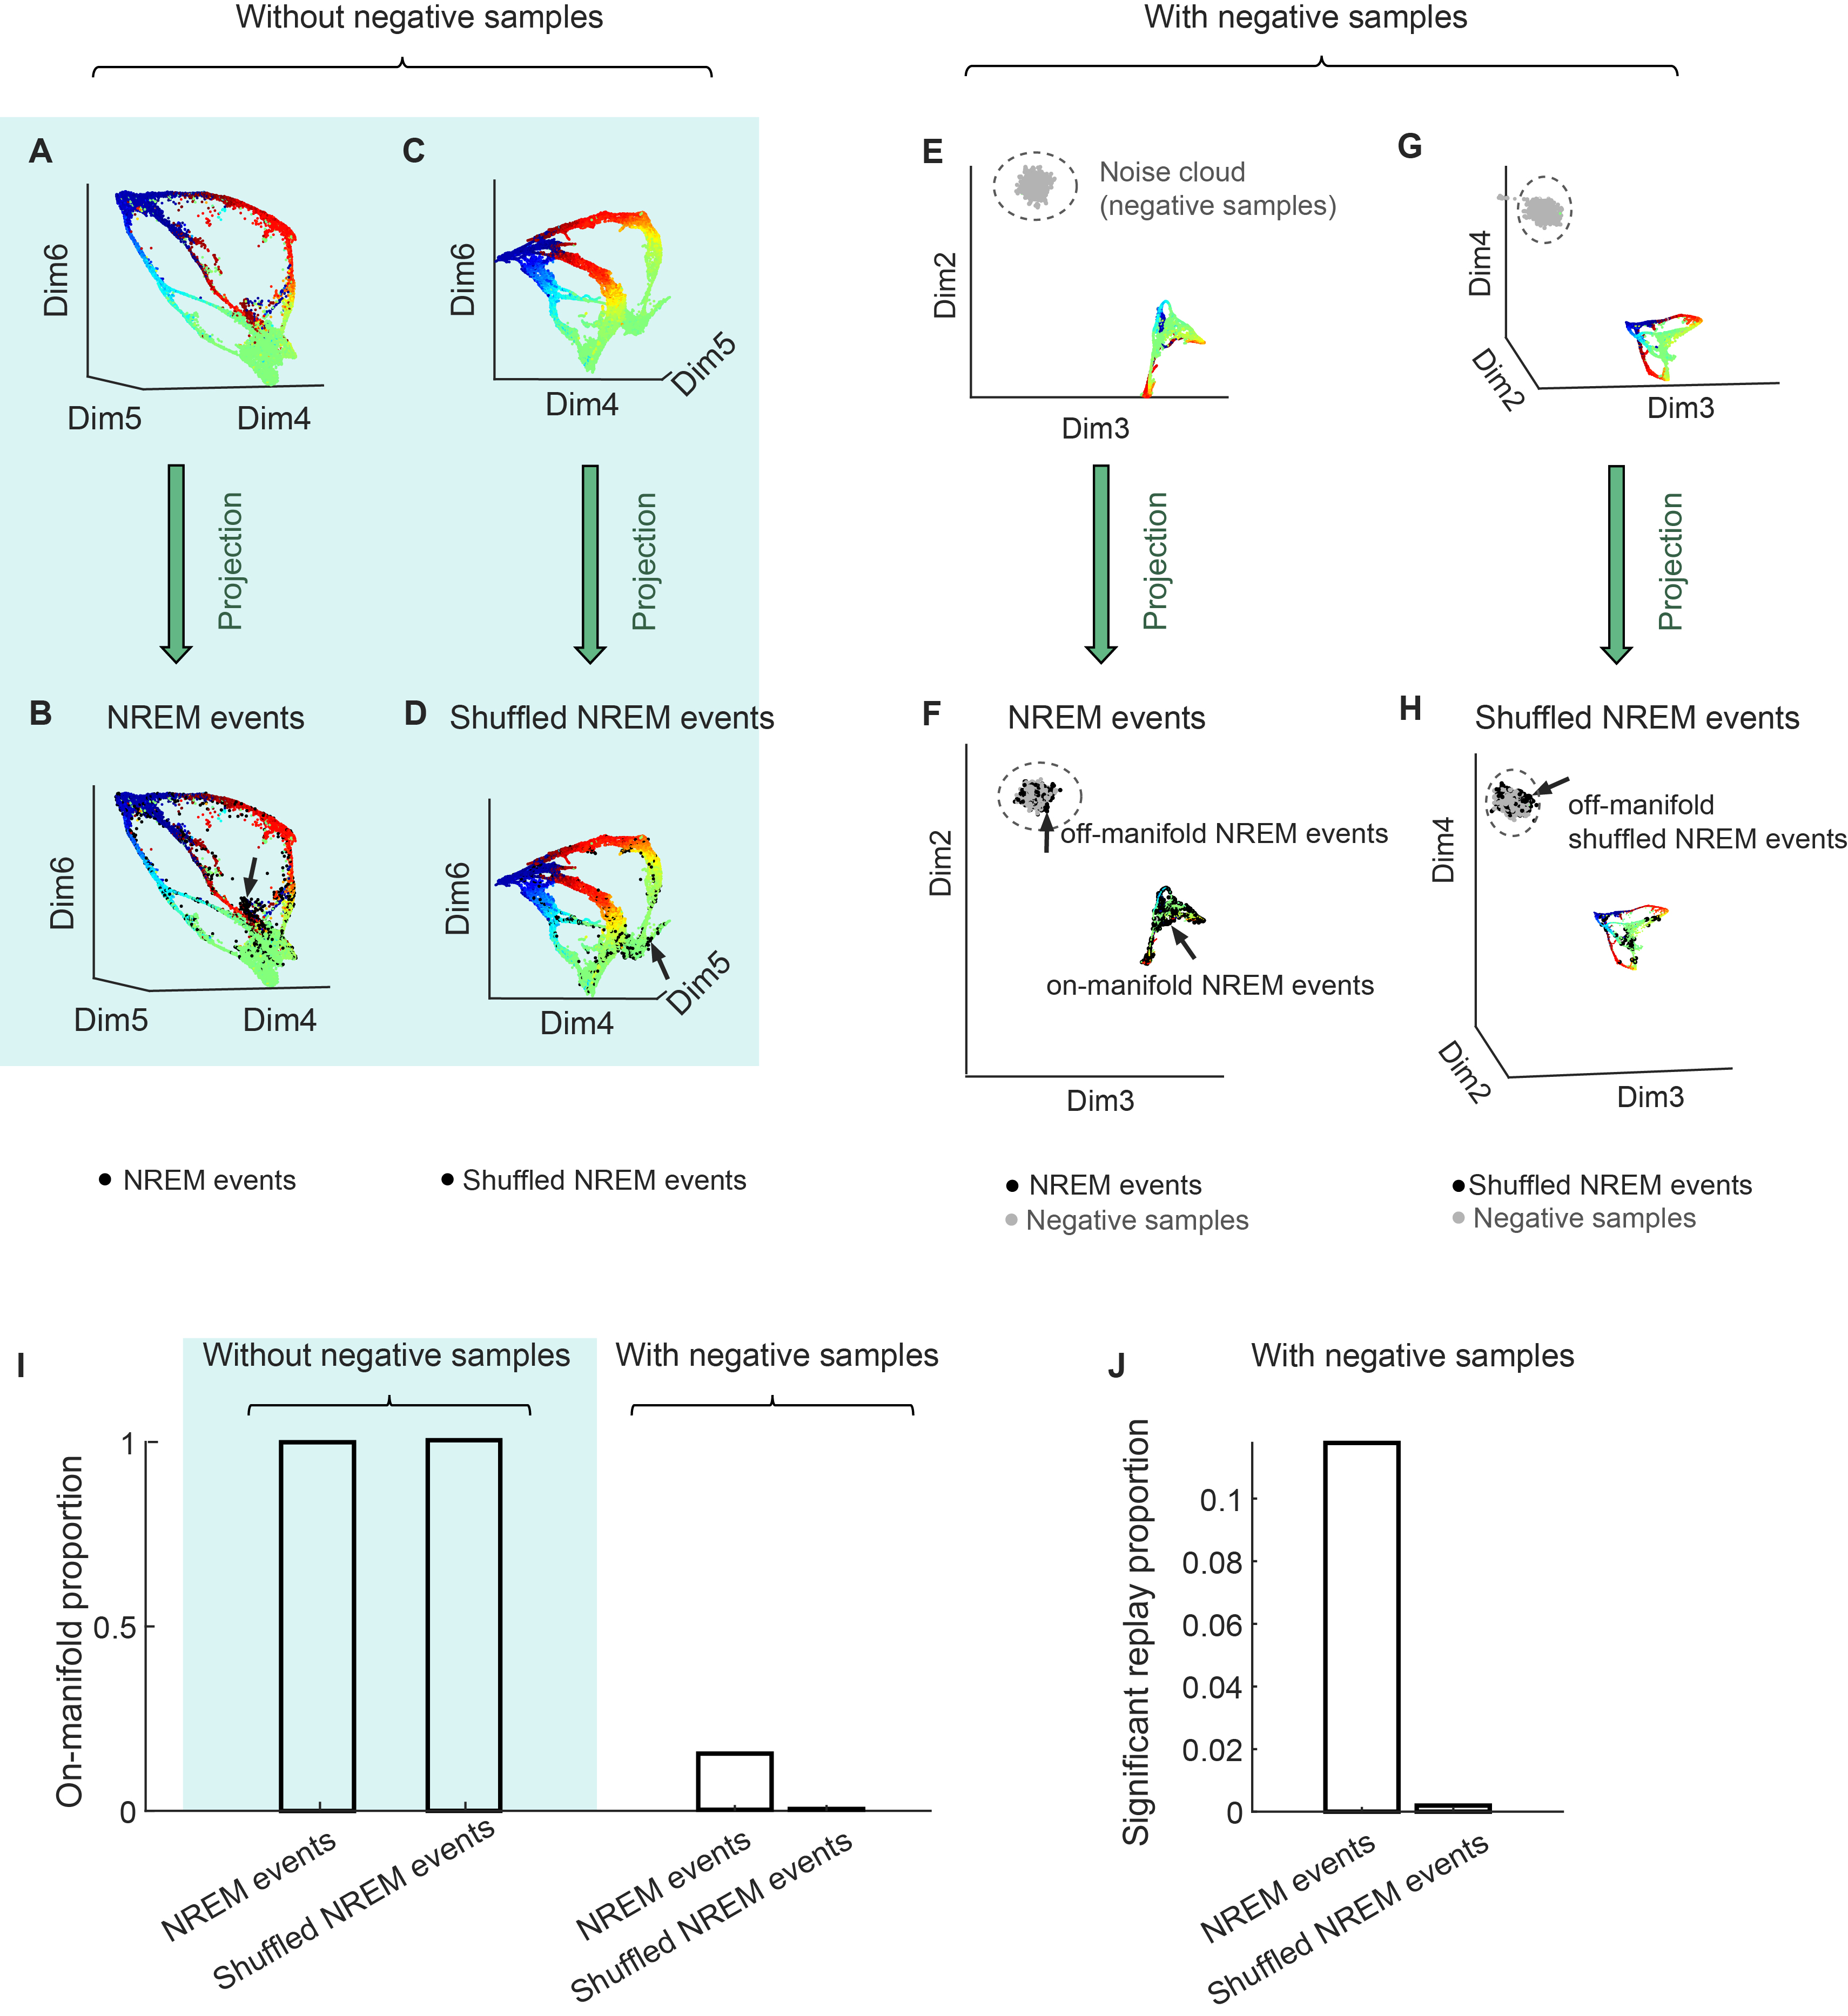
\includegraphics[width=\textwidth]{figures/ch_nreps2023/figB1.png}
    \caption[Metric learning and negative sampling for replay classification]{%
    \textbf{Metric learning and negative sampling for replay event classification.}
    This figure relates to Step 5 of the decoding procedure in Figure~\ref{fig:nreps_appA1}. Candidate SPW-R events are classified as significant replay events only if their distance to manifold and trajectory length are significantly small compared to null distributions.
    \textbf{A.} Shuffling procedure for degrading temporal information of candidate SPW-R events without changing other properties of population activity (preserving relationship across rows). This is done by shuffling cell ID. This procedure generates shuffled events with long trajectory length compared to true replay events without affecting distance to manifold.
    \textbf{B.} Temporal shuffle. This procedure degrades the population activity pattern while preserving temporal information of SPW-R events by shuffling the rows of the spiking matrix (preserving relationship across columns). This generates shuffled events with large distance from manifold compared to true replay events, without affecting trajectory length.
    \textbf{C.} Middle: scatter plot of events in a 2D metric defined by the z-scored distance to manifold and trajectory length. Bottom: histogram for distance to manifold comparing shuffled data (grey) and all SPW-R events (red) in an example session. Left: histogram for trajectory comparing shuffled data (cyan) and all SPW-R events (red).
    \textbf{D.} Zoomed-in display of significant replay events. Black dashed line, significant distance threshold. Red dashed line, significant trajectory threshold.
    \textbf{E.} Density plot of SPW-R event distribution, where density value is the z-scored count of events in each cell of a 30$\times$30 grid of the distance-trajectory metric.}
    \label{fig:nreps_appB1}
\end{figure}

\clearpage

\subsection*{Appendix C: Quantifying Significant SPW-R Replay Events Against Shuffle Events}
\label{app:nreps_C}

\begin{figure}[htbp]
    \centering
    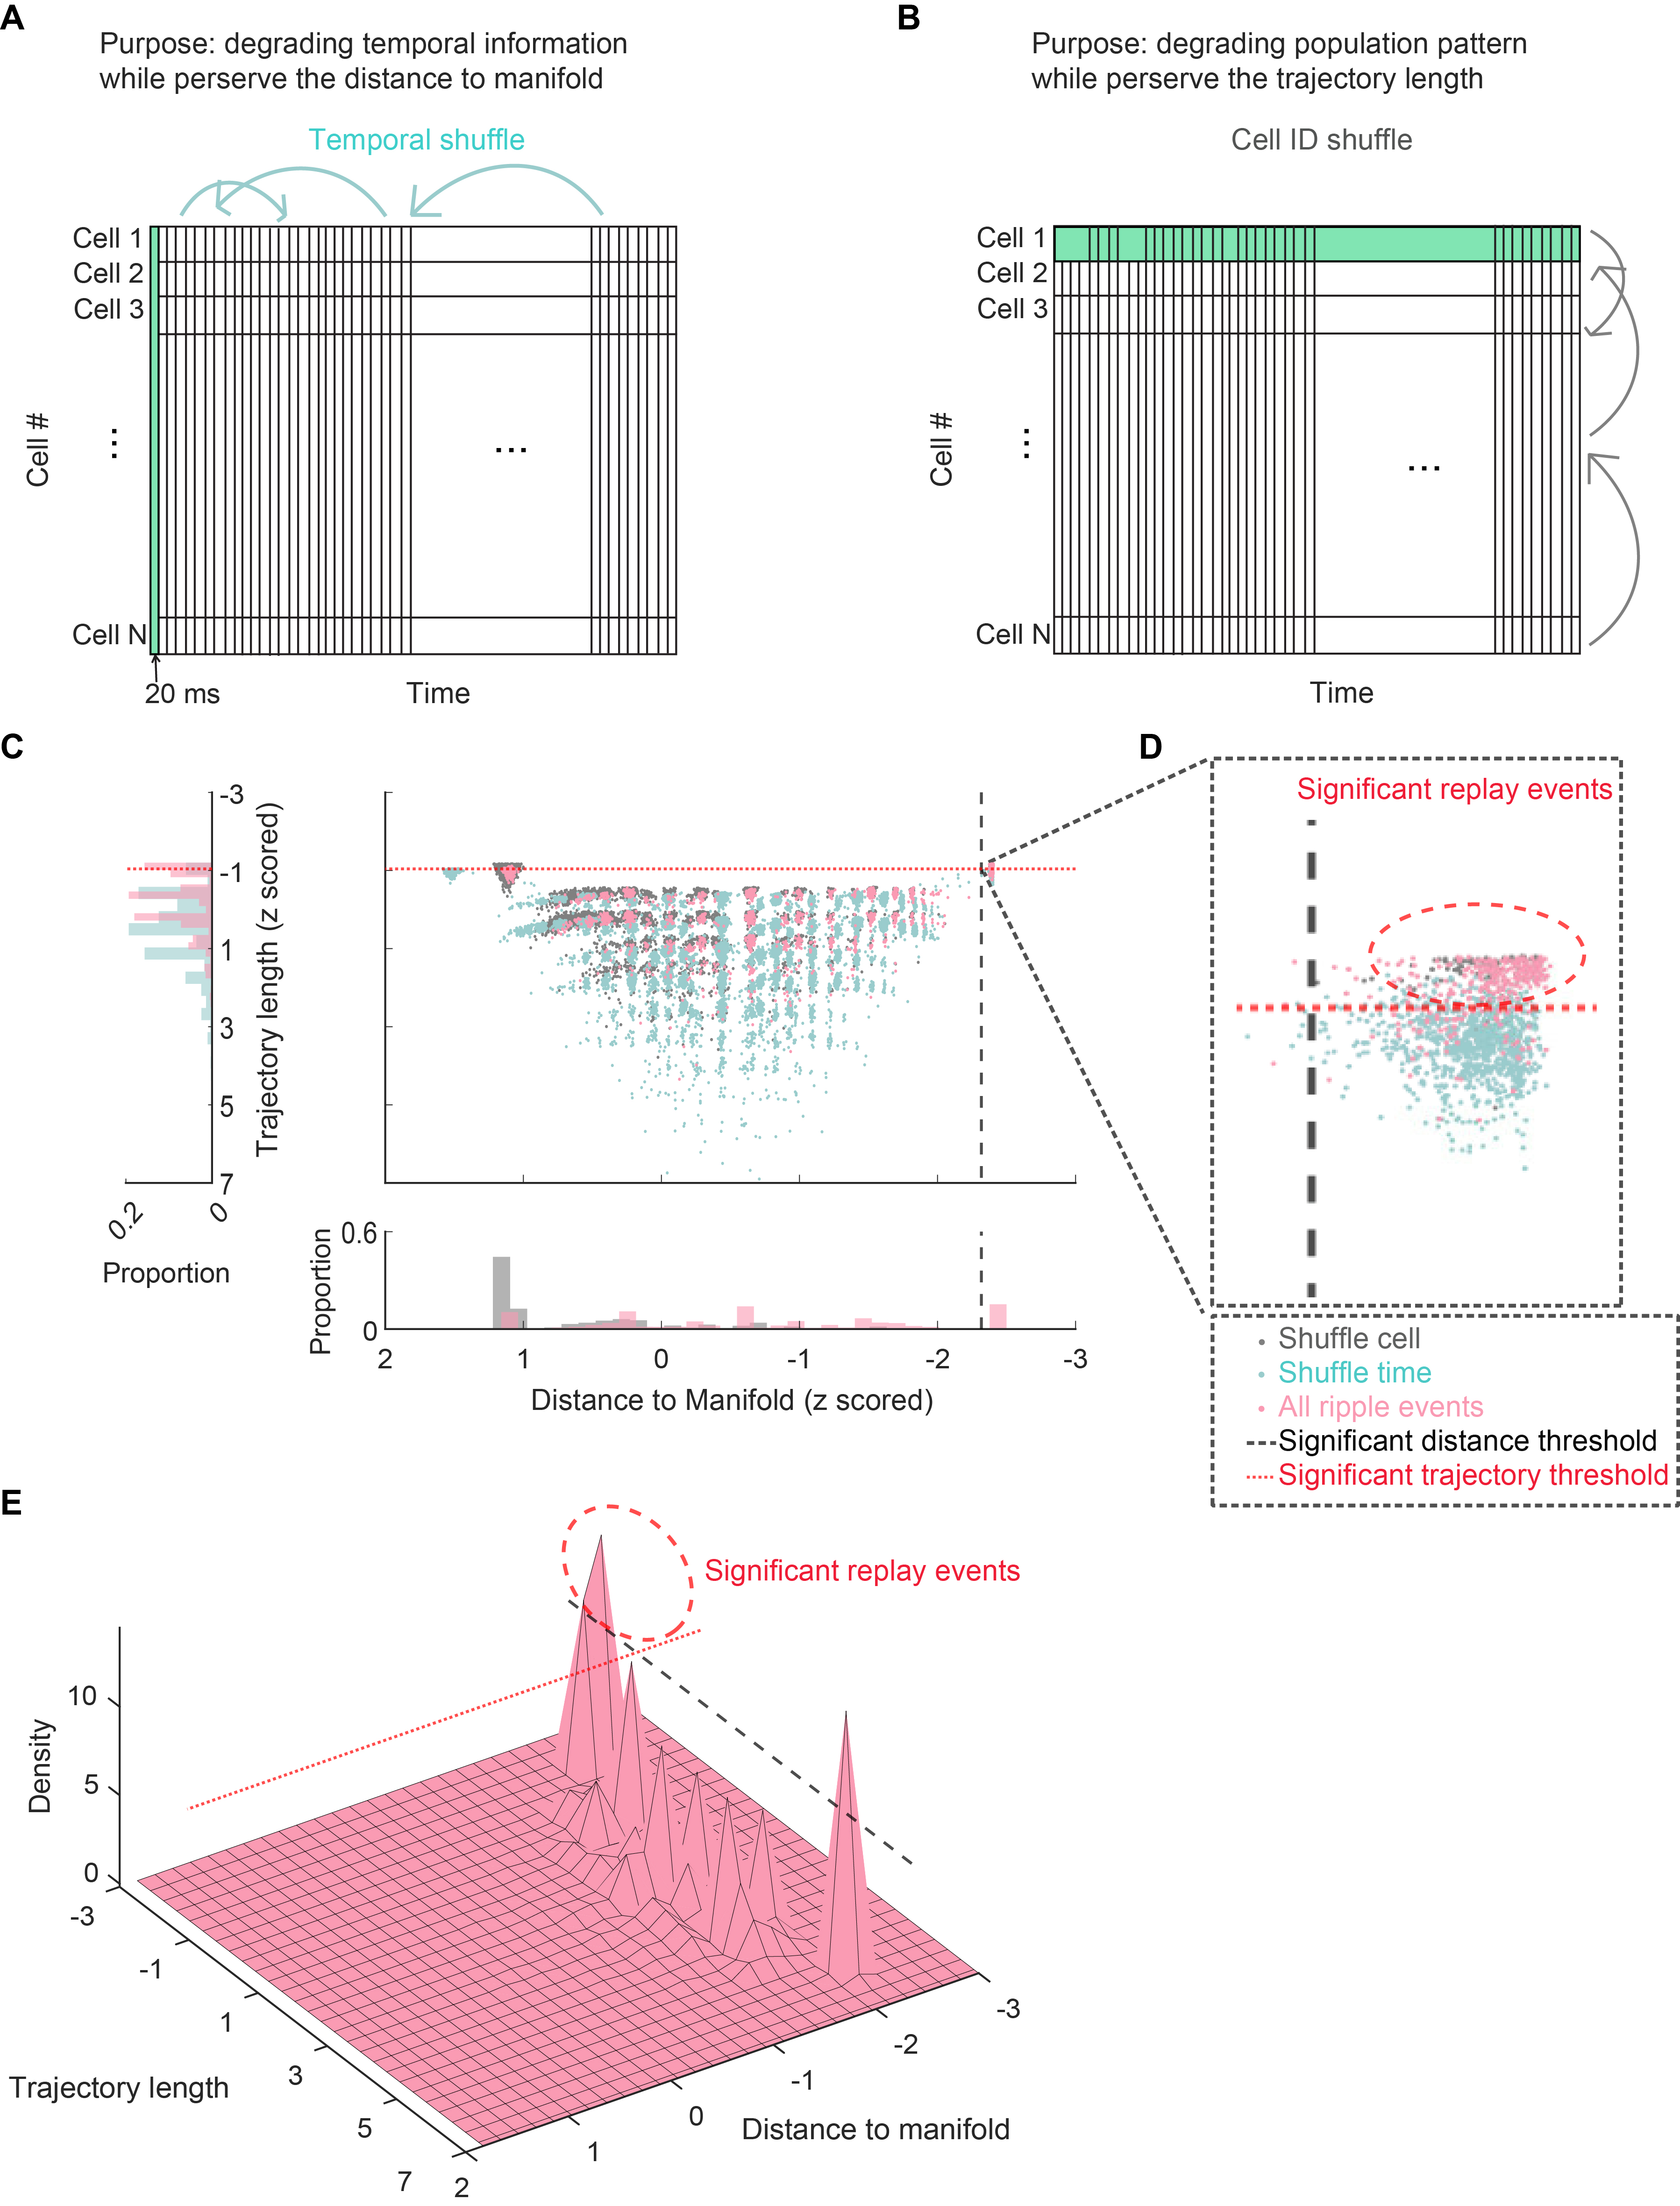
\includegraphics[width=\textwidth]{figures/ch_nreps2023/figC1.png}
    \caption[Quantification of significant SPW-R replay events against shuffled distributions]{%
    \textbf{Quantification of significant SPW-R replay events against shuffle events.}
    The proportion of events classified as significant replay events is shown separately for awake sharp wave ripples (SPW-R), NREM sleep SPW-R, and REM sleep SPW-R, alongside their respective shuffle distributions. The fraction of significant REM replay events is not statistically different from that of shuffle events, in contrast to NREM sleep where significantly more events than chance are classified as significant replays. This analysis establishes that NREM sleep, but not REM sleep, contains robust replay of the recent awake experience using the unsupervised manifold-based decoding approach.}
    \label{fig:nreps_appC1}
\end{figure}
